\chapter{Implementation} \label{implementation}
This chapter will discuss the implementation. It presents all implemented solutions ranging from brute force exact pattern matching \ref{bruteepm} and approximate pattern matching \ref{bruteapm} up to exact solution using skipping dimensions \ref{bynepm}, approximate algorithm using dynamic check \ref{ffsapm}, algorithm using preverification phases \ref{sfapm} and solution using various hash functions \ref{hsfapm}.

Primary languages were C++ and Python. For compilation of *.cpp programs user needs at least compiler of version 2011 (flag \texttt{-std=c++11}). All Python scripts were run using version 3.0. A \textit{numpy} library is also needed. A~\textit{Makefile} was created in order to simplify the C++ compilation.

Libraries used in C++ were iostream, fstream, string, vector, math.h and chrono which are all included in the C++11 standard.

\section{Input Data}
A large part of the database search revolves around used data structures, so this section will focus on the specifications of used formats and other properties. For this task three Python scripts were implemented and their usage and descriptions are in the sections below focused on generating of data \ref{generating}, data filtering and chunking \ref{chunking}, all of these scripts expect CSV data as input format, because it is one of the most common data storage format. However first section \ref{format} is explaining input data format which the scripts can process.

\subsection{Real datasets}
Implementations were also tested using some real datasets \footnote{Provided by \url{archive.ics.uci.edu/ml/datasets}}. However there is a need of preprocessing of the data, as they are missing proper headers. The chunking can be done by the provided script. After these operations the datasets can be used the same way as testing data.

\subsection{Format}\label{format}
Data format (file extension) that can be successfully processed is of types CSV and BIN where CSV data must have a header in the format:
\begin{itemize}
\item 0:DIMX$_0$, 1:DIMX$_1$, \ldots , N:DIMX$_N$, ATTR1:TYPE, ATTR2:TYPE, \ldots , ATTRL:TYPE
\end{itemize}
In this format $(0, N)$ is an order of the dimension whilst $(X_0, X_1, \ldots , X_n)$ is a number of unique values that are in this dimension. $(ATTR1, \ldots, ATTRL)$ specifies the name of the attribute and TYPE parameter contains the type of the values in the attribute, only one type per attribute is allowed. 

Various examples of this format can be: 
\begin{itemize}
\item 0:DIM5, 1:DIM5, 2:DIM5, TIME:FLOAT - this data has three dimensions where each of them contains 5 values and one attribute named TIME using type float.
\item PLACE:DIM3,TYPE:DIM4,PRIZE:INT - this could be a specification of races where there are three different places, four different types and the prize for the winner is specified in attribute PRIZE.
\end{itemize}

When the user needs binary data, another script can be used to create chunked and binary data from the original CSV file. This script is specified in the section called Chunking \ref{chunking}.

Following this specific header are usual CSV data. Be aware that the data can be sparse, which means there can be missing cells or attributes.

\subsection{Generating Data}\label{generating}
Data generating is taken care of by two scripts where both of them generate hyper-cubic data (this is a simplification for the analysis of the algorithms, although algorithms can be used for different lengths of dimensions and patterns). First of them will generate data where no cell is missing or NULL value.
When in need of sparse data, second script named can generate them with the help of multidimensional Gaussian functions. 

The actual generating is based on random generated three Gaussian distributions with the centers set in three different positions

An example of generating data in two dimensional space is in the figure \ref{gauss} where the ellipses $G_1, G_2$ and $G_3$ represents where the data are going to be generated, $S_1, S_2$ and $S_3$ are the centers of the ellipses.


\begin{figure}
\centering
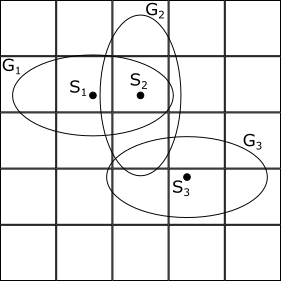
\includegraphics[width=0.5\textwidth]{gauss}
\caption{Example of the space filling with Gaussian functions. \cite{mdApproxPM}}
\label{gauss}
\end{figure}

For pure testing purpose there is also a script which is prepared for creating patterns at specific positions of the data.

\subsection{Chunking}\label{chunking}
All tested data are represented in binary format and chunked into files which represent a set number of cells based on the dimension sizes.

Attribute values are added into the relevant file, which is determined by the dimension values. Created files have their names same as the input file with the dimension numbers added to signify which data are stored in them. For example, if the input data are two dimensional, there are two possible options to perform chunking based on the size of the data and maximal chunk size. First, if the data are small enough, the chunking would use only one bin file. Otherwise, for each ``row'' a single bin file would be created to easily determine what data are stored in them.

As was already specified SciDB has its own binary format and the chunking uses exactly the same format. This means there is always one special file with meta information about the chunked binary files. In meta file there can be found header of the original data as this file is not binary encoded. There is also a mask file that specifies if a cell is in the data or not by using one bit per each cell (0 means the cell is not in the data and vice versa). Other files created by the script are of a binary type that contain a sequence of cell values. For the sake of testing attributes were only of integer type, but implementation can also work with other values.

The main advantage of the chunking is that the algorithm does not need to hold all data in the memory and instead read only currently processed sections.

\section{Output Format}
After successfully running the executables in the terminal window the program will write in the standard output stream. First it will write Finding, meaning that the part of the program that searches for solutions started and all initial settings and reads are done. When finished with find phase program will output the time it took to find the results and after this it will write coordinates of the found solutions. They will be written in the form of list of all possible dimension coordinates where the desired pattern can be found while not violating the constraint about maximum number of errors.

Usual output would contain an array of found solutions, however as this work is concerned about the process of finding, the result serves mostly a~confirmation role. If the algorithms were used in real system, it would be simple to modify the output to suit the system needs.

\section{Pattern Matching}
In this section eight implemented solutions of pattern matching are presented. First part \ref{epm} is focused on two solutions used for solving of exact pattern matching, and second part \ref{apm} is dedicated to approximate algorithms.

\subsection{Exact pattern matching}\label{epm}
Every other algorithm is a type of pattern matching. This section will present implemented exact solutions. Exact pattern match means there are no errors and the pattern is present in the data without changes. Two solutions were implemented as reference solutions. First of them is solution using naive brute force algorithm. Second is algorithm by Navarro which skips first dimensions and thus have smaller both patterns and data to compare.

\subsubsection{Brute Force} \label{bruteepm}
As the name suggests this algorithm goes through every position in data and starts to compare the pattern from the ``top-left'' corner until it encounters error. This solution is very simple, on the other hand there is obviously no possibility not to find every position of the pattern.

Just to clarify things, the algorithm iterates over every dimension and in it over every value, thus the returned positions are sorted.

\subsubsection{Baeza-Yates and Navarro modification}\label{bynepm}
This algorithm was proposed by Baeza-Yates and Navarro \cite{mdApproxPM}. Its process is similar to the brute force algorithm, however one dimension which is present in both the pattern and the data is selected. While iterating through this dimension instead of taking steps of length 1, steps of length $m$ are taken.

Not to miss any possible solution, every ``row'' of pattern is compared with the given part of the data. This process is better illustrated in the figure \ref{fig_skipDim}.

Search cost in the worst case corresponds to verifying all text positions the same way as brute force algorithm, which gives $ \mathcal{O} (rm^dn^d)$ where $r$ is the number of searched patterns (in this case $1$), $m$ is the size of pattern in one dimension and $n$ is the size of data in one dimension, for simplicity the algorithms will work only with square shaped data, $d$ specifies the number of dimensions \cite{mdApproxPM}.

\begin{figure}
\centering
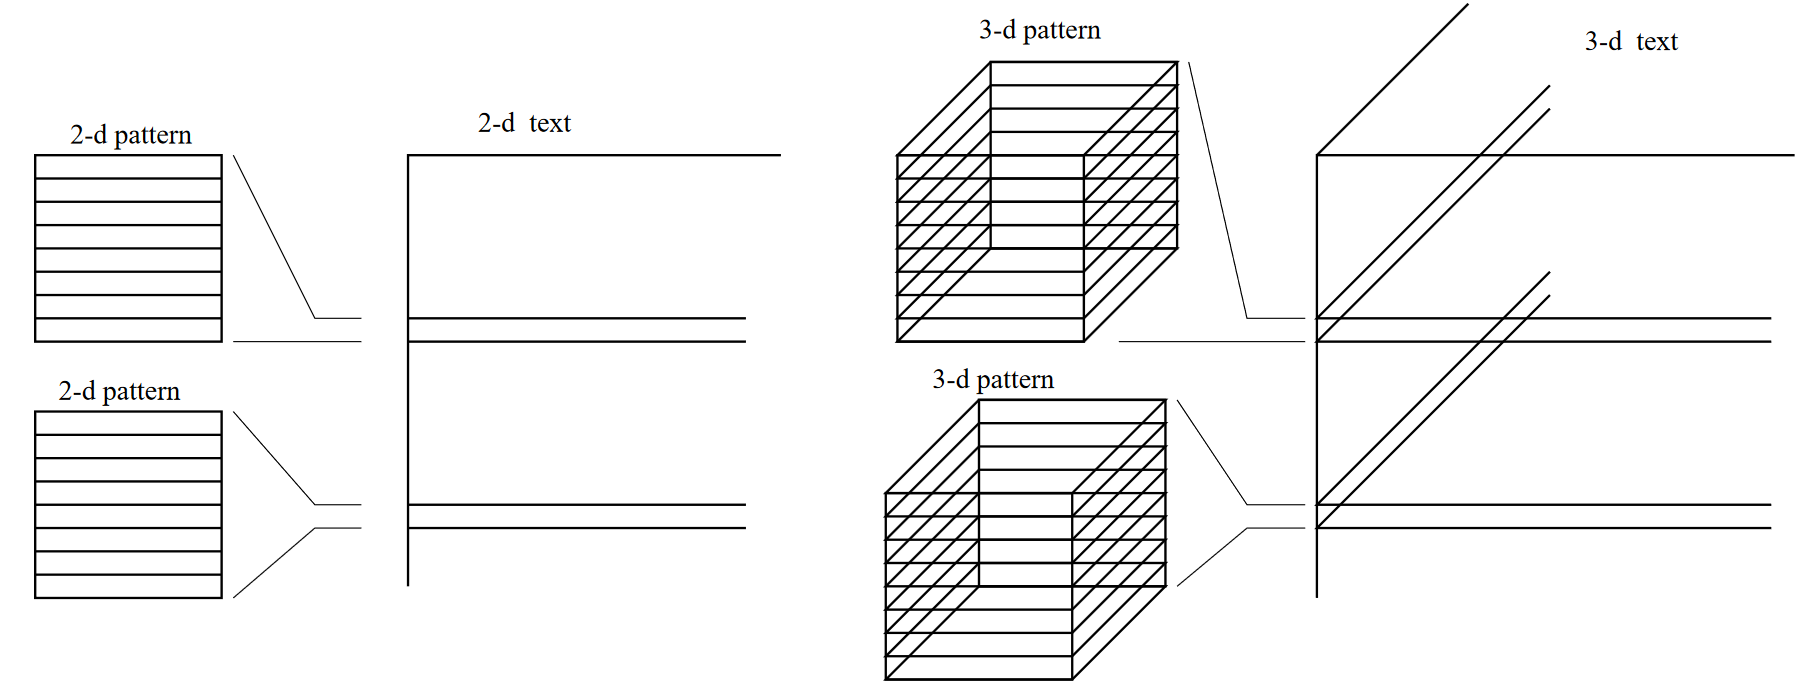
\includegraphics[width=\textwidth]{skipDim}
\caption{Illustration of comparison between pattern and data. \cite{mdApproxPM}}
\label{fig_skipDim}
\end{figure}

Considering that both pattern and data have all dimensions with the same sizes and the selected dimension is arbitrary, the first one is always used for easier implementation. This modification reuses parts of data instead of using every single cell.

\subsection{Approximate pattern matching} \label{apm}
Previous two solutions could us a simple identity function to recognize, whether the solution is valid or not. If an approximation is taken into account, the algorithm has to measure the difference between the pattern and the currently tested position. There exist several options to do that. In the next section all implemented variants are presented.

In every solution an input value $k$ is added, which represents the maximal tolerated error.

\subsubsection{Brute Force}\label{bruteapm}
First and again the simplest solutions to iterate over every part of the data and compare one coordination of the pattern of another until either whole pattern is checked or the $k$ number of errors are found.

This method obviously always finds every valid solution so the number of False Negatives is 0. However it is linearly dependent on the selected error, so it is not suitable for large patterns with higher error range. On the other hand, the implementation is very simple again and it serves as a solid confirmation of the correctness of other solutions.

\subsubsection{Fast Filter Searching}\label{ffsapm}
A less demanding solution was proposed again by Baeza-Yates and Navarro \cite{mdApproxPM}. Its idea is similar to the modification made in the exact algorithm, however in this case an iteration in all dimensions present in the pattern are influenced.

The data are divided into sections, which are the same size as the pattern. The iteration through positions in dimensions not present in pattern is the same as in brute force algorithm. However in the other dimensions, both the section of data and the pattern is divided into the same number of parts and the comparison is made only between the ``bottom-right'' corner of data section and all pattern parts. Not to miss any possible positions, the compared part of the data has to be moved always by one cell part size - 1 times. Again, for better illustration a figure \ref{fig_slide} is provided. In the picture length of the pattern is 10 and is split into two parts. Each part of the pattern is then compared with the ``bottom-right'' corner of the section and then with the parts moved by one until the compared part would not be overlapped with the first part as shown in the figure.

\begin{figure}
\centering
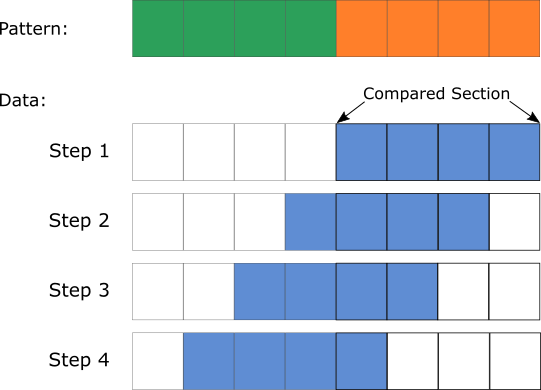
\includegraphics[width=0.6\textwidth]{slide}
\caption{Example of sliding window.}
\label{fig_slide}
\end{figure}

In current implementation all dimensions are split into $m$ parts, except the last, which is split into $j$ parts, where:

$$j = \lfloor k^{\frac{1}{d-1}} \rfloor + 1$$

this value is recommended, so it was not tampered with. This relatively small parts are compared by basic identity function and the positive results are remembered. The whole process usually returns more results than it should, because only a small parts of the pattern are matched. So further verification is needed.

In this case a dynamic programming method is utilized. To perform the dynamic programming check, multiple approaches are available. Completely implemented and tested was only Edit distance, with framework prepared in code for R, C and RC measures as specified in section \ref{similMeasures}. Following methods also use this step, so the dynamic programming was reused.

Usually the dynamic programming confirmation would be made right after finding each position. However considering that all implemented algorithm use chunked data and thus not every section of the pattern is necessarily in the memory, these stages are split and the whole data are searched through for the partial matches and after that the dynamic programming check is performed on all found positions.

When using the ideal $j$ value, the total cost of search and verification is: $$n^dk^{\frac{d}{d-1}}\Big(\frac{1}{m^{d-1}k^{\frac{1}{d-1}}} + \frac{1}{\sigma^{m/k^{1/(d-1)}}} + \frac{d!m^{2d}}{\sigma^{m^d/k^{d/(d-1)}}}\Big)$$ as stated in \cite{mdApproxPM}, where $\sigma$ is the cardinality of the alphabet. This algorithm is then sublinear for the number of errors $$ k < (m/(d \log_\sigma m))^{d-1} $$ and it is not sublinear but still better than dynamic programming for $$k \leq m^{d-1}/(2d\log_\sigma m)^{(d-1)/d} $$

Expected cost of verification the third addend while the elements before express the cost of the find phase. For more informations and explanation of course of action leading to this formula see \cite{mdApproxPM}.

Concerning number of False Positives and False Negatives, the verification phase should prevent the existence of False Positive results. This also applies to algorithms Stricter Filter and Hashed Stricter Filter explained in the next sections. However, there is a possibility of False Negatives because the algorithm requires strict match of a specific part, which in reality could be just the part with the allowed error.

\subsubsection{Stricter Filter}\label{sfapm}
A slightly modified version of previous method is called Stricter filter and was proposed in the same paper. The disadvantage of previous solution is, that if the first partial matching finds a large number of False Positives, the dynamic programming is then a bottleneck, because it is computationally expensive to perform.

Therefore, before the last stage a preverification step is added. It has the same goal as the dynamic programming, however is much simpler and thus much faster. It should filter a large portion of results, which will not be necessary to go through by the dynamic programming.

The idea is to check the found area cell by cell and remove it from solutions if more than $k$ are found. The preverification can end before iterating through all cell if:

\begin{enumerate}
\item $k+1$ errors are found, i.e. the position is not a solution.
\item Less than $k - q$ cells remain to compare, where $q$ is the number of already found errors.
\end{enumerate}

New search cost is then: $$ n^d \Big(\frac{j^{d-1}}{m^{d-1}} + \frac{j^d}{\sigma^{m/j}} + \frac{j^djk}{\sigma^{(m/j)^d}} + \frac{{j^d \choose jk} d! m^{2d} }{\sigma^{m^d - km^d/j^d -1}}\Big) $$

which is the sum of all steps in this algorithm: find phase (first two parts), preverification phase (third addend) and dynamic check phase (last addend).
\subsubsection{Hashed Stricter Filter }\label{hsfapm}
All of the previous approaches were either the simple obvious solutions or previously proposed by Baeza-Yates and Navarro. The last solution is built upon the Stricter Filter and modifies one significant feature. The problem with Stricter Filter solution is, that there has to be the partial identity for arbitrary error value.

So instead of using the comparison of the actual sections of pattern with the data a hash function is implemented. Firstly, all parts of the pattern are hashed, so it is done only once. The same cannot be done with the whole data as only some parts should be hashed and the data are not loaded at the start as they are chunked in smaller files.

Three similar solutions are presented and each of them will be individually presented in its own paragraph below. The rest of the processes stays the same as in the Stricter Filter, so preverification and dynamic programming check is performed.

The assumption is, that the added hashing may increase the computation speed, because a lot shorter values are compared instead of whole sections. However the part size will have high impact on the improvement, because the higher the ratio between part size and hash size the bigger the improvement. Another possible outcome is to find even more partial results for preverification, because the the hash function will probably make some collisions.

The best case scenario thought is that the collisions will be for similar sections and thus possibly valid positions, which were disregarded by the Stricter Filter method. This is the reason for usage of SimHash, while the use of the other hash function is supported by the idea that when the data are created randomly there is a little chance for the orders of numbers to be repeated and thus creating less collisions.

The complexity of this algorithm is the almost the same as of Stricter Filter algorithm, but the find phase elements are reduced by the probability of the hash reusage.

Number of the created hashes for SimHash and LSB hash discussed in the sections below is:
\begin{itemize}
\item Pattern -- $m^{d-1} * j$
\item Data -- $(\frac{n}{m})^{d-1} * \frac{m}{j}$
\end{itemize}

The number of False Negatives is similar as in the previous approximate solutions with the difference that hashes may return some previously not found positions due to the hash collisions.

\paragraph{Naive SimHash} First implemented variant uses SimHash which is created by hashing attributes needed to compare (attributes present in the pattern) and then combining the partial hashes into one hash where each bit position contains 1 if there is more 1s than 0s in the same bit position of all partial hashes. The hash used for the partial hashing is simple identity as the testing data use only integer values with the highest value of 255, so it is  basically an eight bit number. The actual hashing of data is performed every time a comparison is required between pattern and data. In the table \ref{simHashTab} is an example of the SimHash, with the final value of $00101000$.

\begin{table}[!h]
\centering
\begin{tabular}{| c | c | c  c  c  c  c  c  c  c |}
\hline
i & Value & \multicolumn{8}{c |}{Bit value} \\
\hline
0 & 43  & 0 & 0 & 1 & 0 & 1 & 0 & 1 & 1 \\
\hline
1 & 56  & 0 & 0 & 1 & 1 & 1 & 0 & 0 & 0 \\
\hline
2 & 11  & 0 & 0 & 0 & 0 & 1 & 0 & 1 & 1 \\
\hline
3 & 167 & 1 & 0 & 1 & 0 & 0 & 1 & 1 & 1 \\
\hline
4 & 204 & 1 & 1 & 0 & 0 & 1 & 1 & 0 & 0 \\
\hline
5 & 38  & 0 & 0 & 1 & 0 & 0 & 1 & 1 & 0 \\
\hline
6 & 64  & 0 & 1 & 0 & 0 & 0 & 0 & 0 & 0 \\
\hline
7 & 249 & 1 & 1 & 1 & 1 & 1 & 0 & 0 & 1 \\
\hline \hline
\multicolumn{2}{| c |}{\# 1s:} & 3 & 3 & 5 & 2 & 5 & 3 & 4 & 4 \\
\hline
\multicolumn{2}{| c |}{\# 0s:} & 5 & 5 & 3 & 6 & 3 & 5 & 4 & 4 \\
\hline
\multicolumn{2}{| c |}{Hash:} & 0 & 0 & 1 & 0 & 1 & 0 & 0 & 0 \\
\hline

\end{tabular}
\caption{Example of Naive SimHash.}
\label{simHashTab}
\end{table}

\paragraph{SimHash} Second implementation varies only a slightly from the first one. The data are hashed using SimHash as well, but only once as they are read from the chunked file, and only the parts to be compared. This reduces the number of hash computations, however it requires another matrix to keep the hashes in memory. The main idea for this hash is to be able to reuse once computed hash values instead of creating them again.

\paragraph{LSB Hash} Third solution uses a variation of the least significant bit hash (LSB), but the position of the LSB is moved after every step. This hash is constructed by using this formula: $h(x_i) = A_i\ \&_{bit}\ 2^i$, where $A_i$ is the i-th value to be hashed, $h$ is the the hash function and $x_i$ is the i-th position of the hash. Main drawback of usage of this hash is that only one bit is taken from every value which means for small compared parts (smaller than eight) it will create higher number of collisions. On the other hand, for longer parts, the hash will actually be longer and thus may create less collisions with the drawback of longer comparison (but still not as long as without using any hash).
In the table \ref{hashTab} is an example of the hash, with the final value of $10000111$.  
\begin{table}[!h]
\centering
\begin{tabular}{| c | c | c | c |}
\hline
i & Value & Bit value & Hash \\
\hline
0 & 43 & 0010101\textbf{1} & 1 \\
\hline
1 & 56 & 001110\textbf{0}0 & 0 \\
\hline
2 & 11 & 00001\textbf{0}11 & 0 \\
\hline
3 & 167 & 1010\textbf{0}111 & 0 \\
\hline
4 & 204 & 110\textbf{0}1100 & 0 \\
\hline
5 & 38 & 00\textbf{1}00110 & 1 \\
\hline
6 & 64 & 0\textbf{1}000000 & 1 \\
\hline
7 & 249 & \textbf{1}1111001 & 1 \\
\hline
\multicolumn{3}{c |}{} & 10000111 \\
\cline{4-4}
\end{tabular}
\caption{Example of Modified LSB hashing.}
\label{hashTab}
\end{table}

This explanation uses an assumption, that each cell contains only one integer attribute, in the actual implementation, the hashes for each attributes are concatenated. 

\section{Possible modifications}
Some other modifications were considered and two of them were analysed, whether it could have a positive impact on already implemented solutions. First modification consist of changing the comparison between the section from the naive algorithm to KMP as the sliding part of the data may be considered as a longer array and the comparison could return only a position in the slide. However considering that the compared sizes are $\frac{m}{j}$ and $2\frac{m}{j} - 1$, and the non-repetitive type of data, the creation of the extra table as specified in \ref{KMP} would add another space requirement and the speed increase would probably not occur, because mostly, the check ends after single value comparison. If these methods were used data, where a repetition of subsequences was expected and the part size was set to sufficient value, it may prove to be faster.

Second modification was to use hashing even for preverification phase. As the pattern was already hashed it seemed as a viable option. However only a~very small portion of the data is hashed at the start of the preverification, as only a few sections are used in comparison and also some of the hashed parts were overwritten in cache. Creating hashes for all required parts of the data would take more time than the actual preverification in current form, so it was not used. If the data were for some reason hashed before, the idea could prove more plausible. For example, if some form of indexing was used.
